\subsection{Wichtige Berechnungen}
Mit der Benutzung und der Anwendung der schrägen Wurf Formel, könnten wir die Geschwindigkeit ausrechnen und damit die notwendige Energie, 
die der Ball braucht um bis zum Korb zu fliegen. Für die Berechnungen haben wir festgestellt, dass wir von ca. 40 cm Höhe abwerfen werden 
mit ein Winkel von ca. 50°. Für die Berechnungen wurde auch ein Rad mit ein Durchmesser von 15 cm benutzt. \\

\begin{figure}[h!]
	\begin{subfigure}{.5\textwidth}
		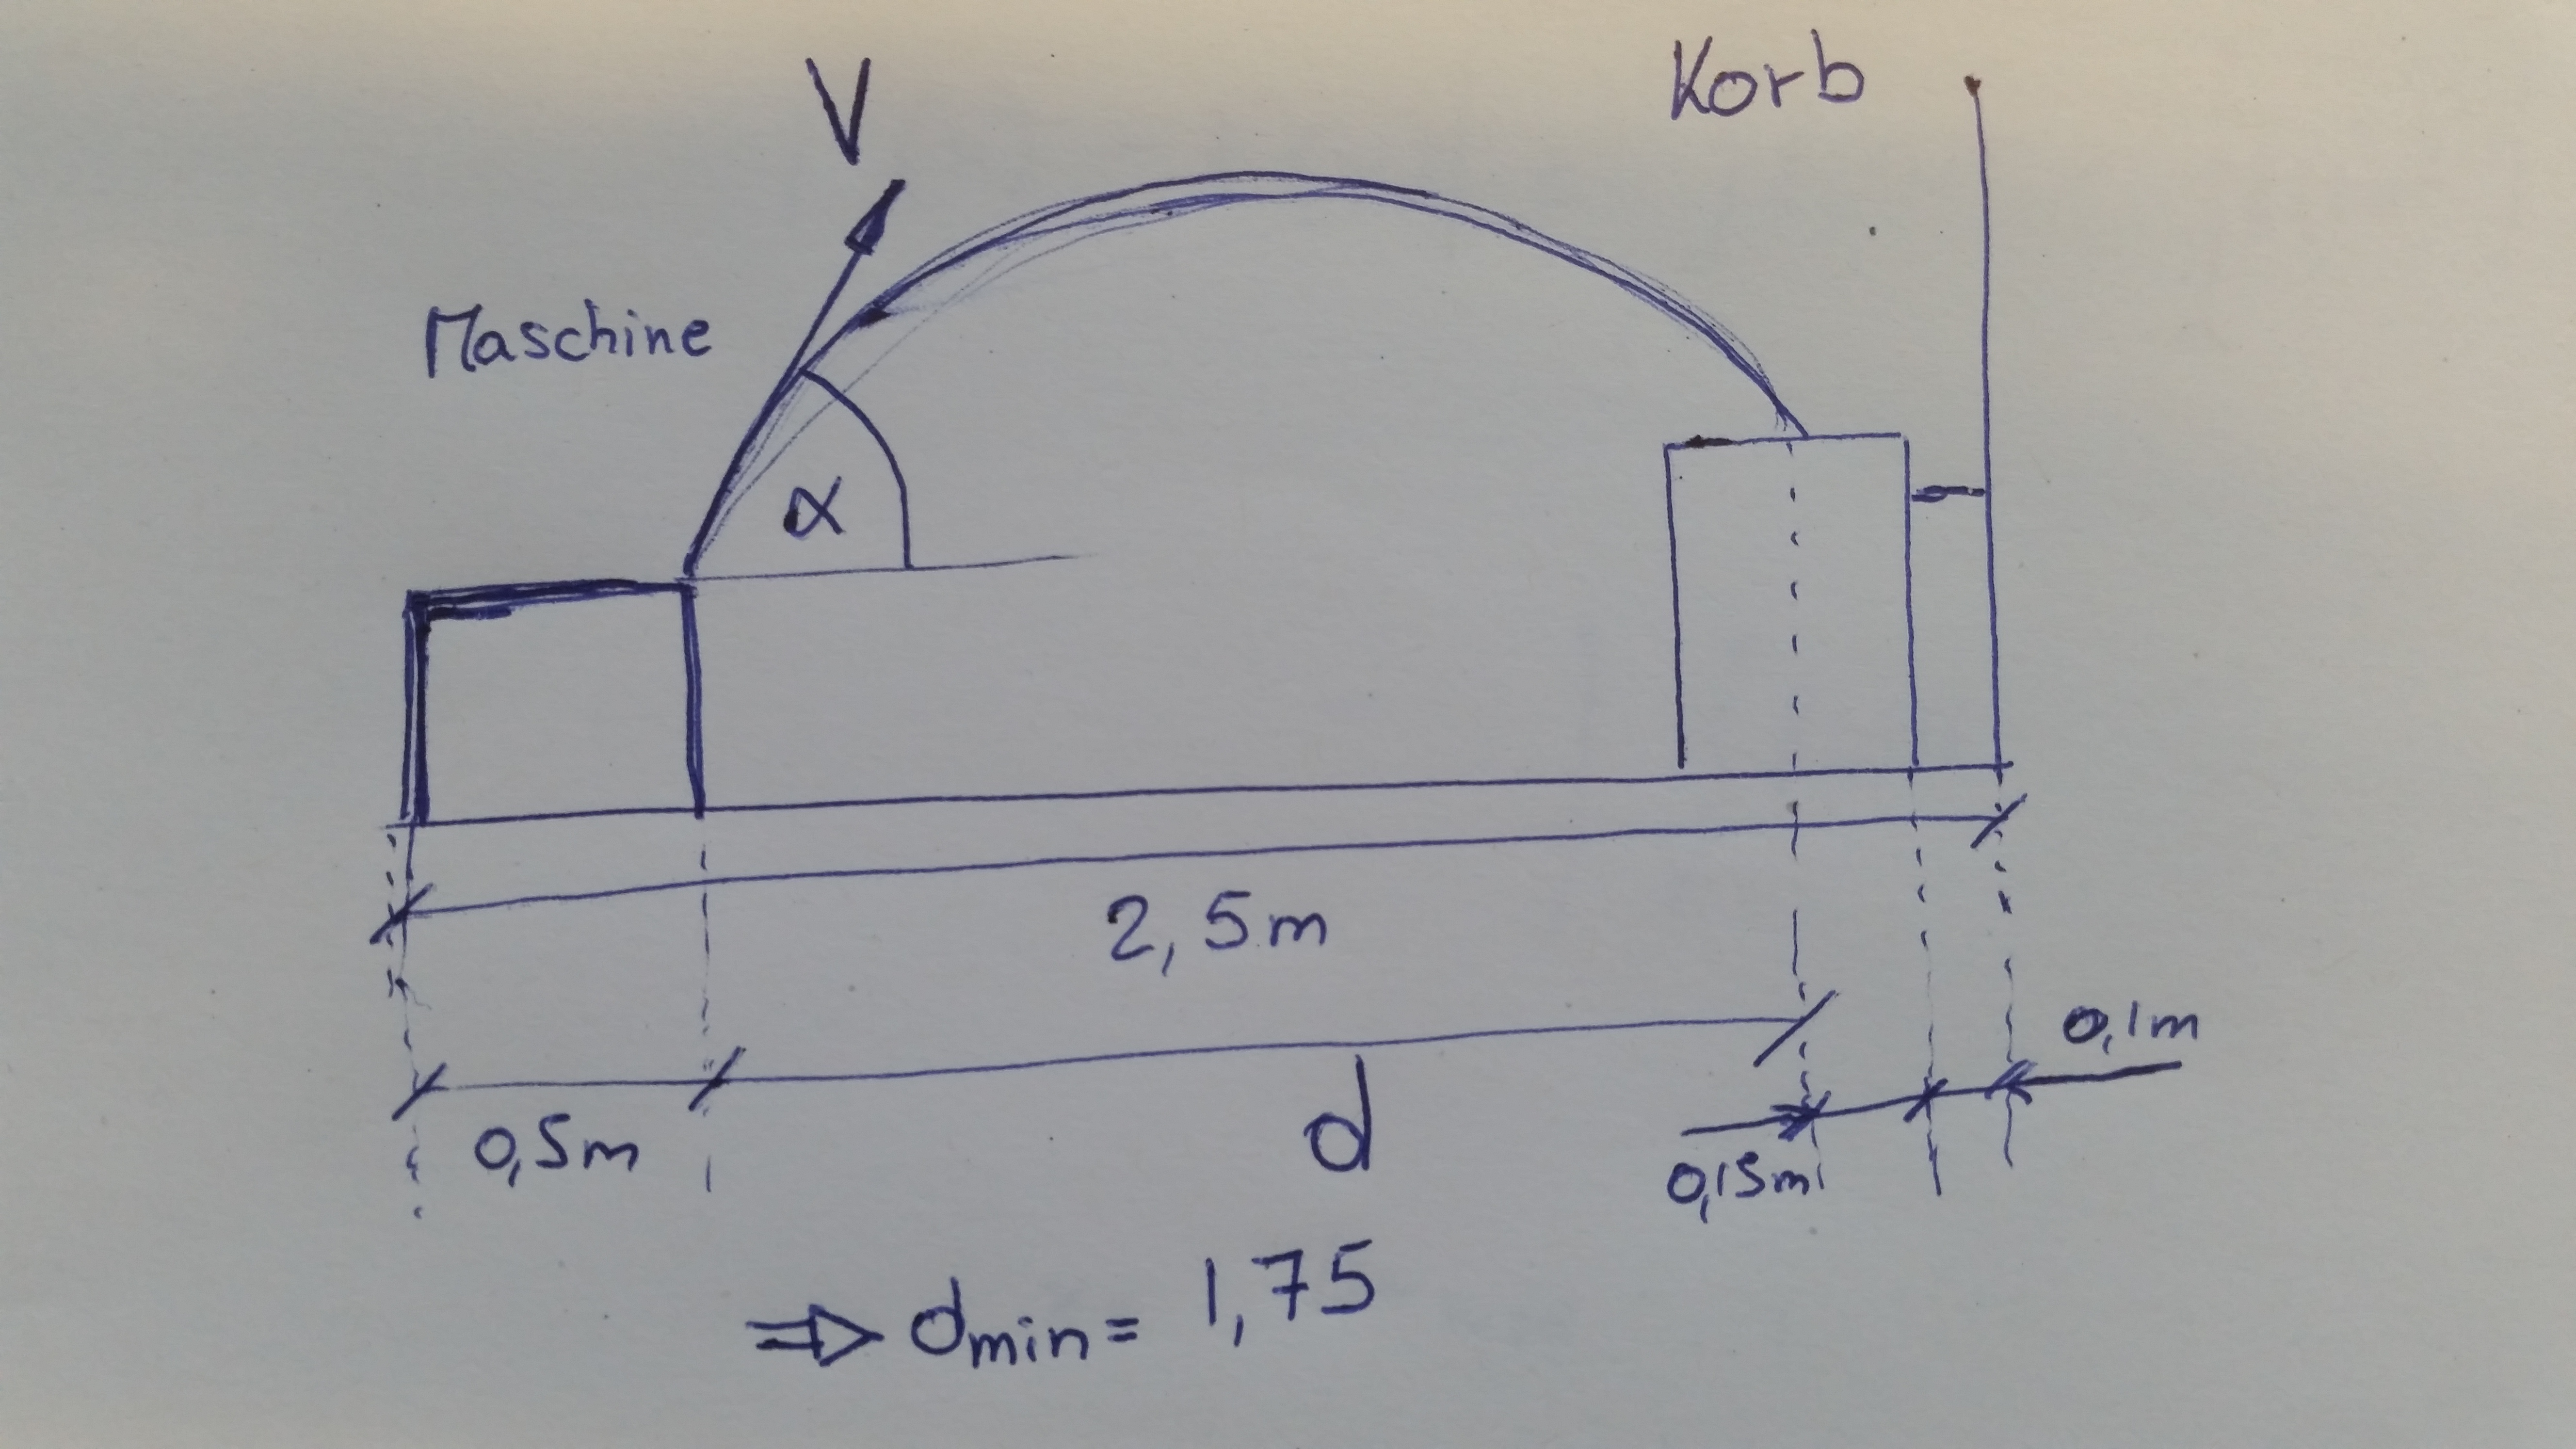
\includegraphics[width=1\textwidth]{../../fig/Skizze_Berechnung_1.jpg}
		\caption{Schrägen Wurf von der Seite}
		\label{fig:Berechnungen von die Geschwindigkeit}
	\end{subfigure} %
	\begin{subfigure}{.5\textwidth}
		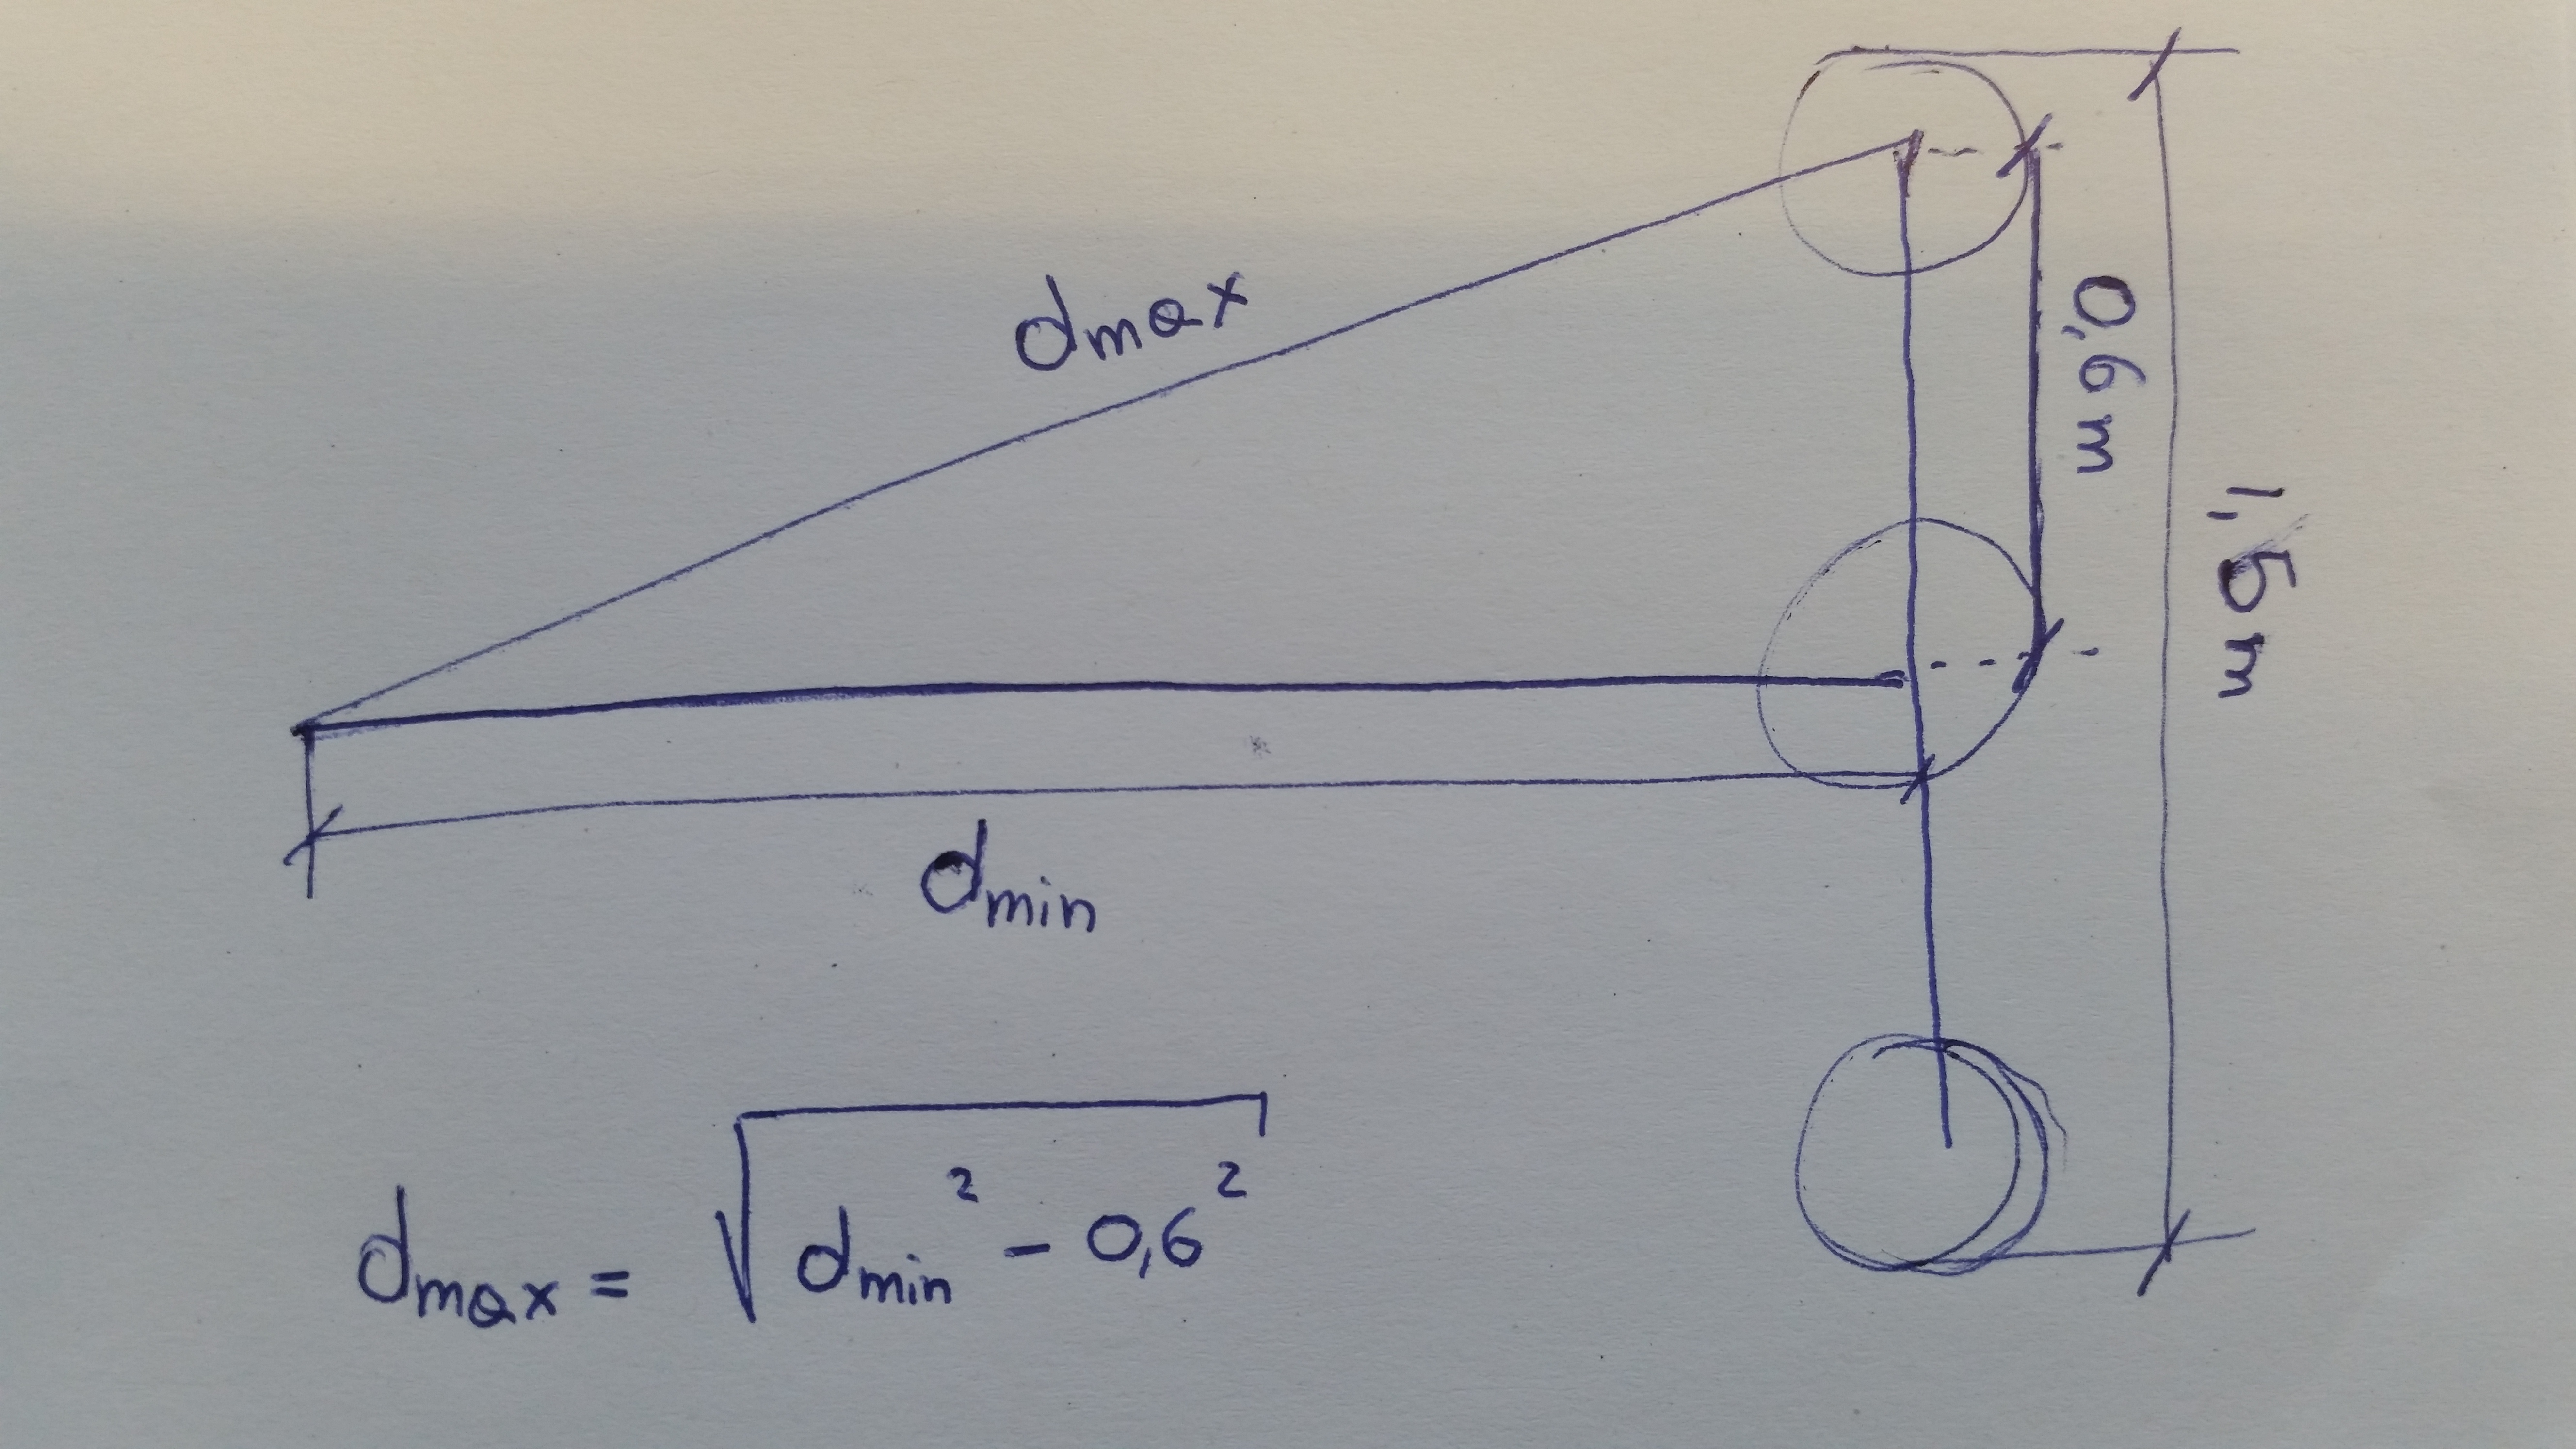
\includegraphics[width=1\textwidth]{../../fig/Skizze_Berechnung_2.jpg}
		\caption{Schrägen Wurf von Oben}
		\label{fig:Berechnungen von die Geschwindigkeit}
	\end{subfigure}
	\caption{Berechnung der Schräger Wurf}
	\label{Berechnungen}
\end{figure}

\begin{gather}
	v=\frac{\sqrt{g}*d}{\sqrt{2}*cos(\alpha)*\sqrt{d*tan(\alpha)+(h_0-h_1)}}\\
	\omega=\frac{v_{tan}}{r}\\
	f=\frac{\omega}{2\pi}\\
	rpm=60*f
\end{gather}

Mit unsere bedingungen ergibt sich eine Geschwindigkeit von 4.18 m/s und ein rpm von 800 U/min bei $d_min$, 
und eine Geschwindigkeit von 4.29 m/s und ein rpm von 820 U/min bei $d_max$. 
Die Abweichung liegt rund um 2.5\%, und wird mid der Steurung der Motor angepasst. \\
Diese Berechnungen sind Rein theoretisch und Faktoren wie Reibung wurden nicht berücksichtigt. Aus diesem Grund werden als Mindistanforderungen behandelt.
